\documentclass[12pt]{extarticle}
\usepackage[utf8]{inputenc}
\usepackage{graphicx}
\usepackage{float}
\usepackage{hyperref}
\usepackage{amsmath}
\hypersetup{
    colorlinks=true,
    linkcolor=blue,
    filecolor=magenta,      
    urlcolor=blue,
    pdftitle={Overleaf Example},
    pdfpagemode=FullScreen,
    }

\title{CS 3600 Project 2 Wrapper}
\author{CS 3600 - Spring 2022}
\date{Due March 6th 2022 at 11:59pm EST via Gradescope}

\begin{document}

\maketitle

\section*{Introduction}

This Project Wrapper is composed of 4 questions, each worth 1 point. Please
limit your responses to a maximum of 200 words. The focus of this assignment is to train your ability to reason through the consequences and ethical implications of computational intelligence, therefore do not focus on getting ”the right answer”, but rather on demonstrating that you are able to consider the impacts of your designs.

\section*{Context}

Reinforcement learning is a powerful technique for problem-solving in environments with stochastic actions. As with any Markov Decision Process, the reward function dictates what is considered optimal behavior by an agent. Since a reinforcement learning agent is trying to find a policy that maximizes expected future reward, changing when and how much reward the agent gets changes its policy. \\

\newpage

\begin{figure}
    \centering
    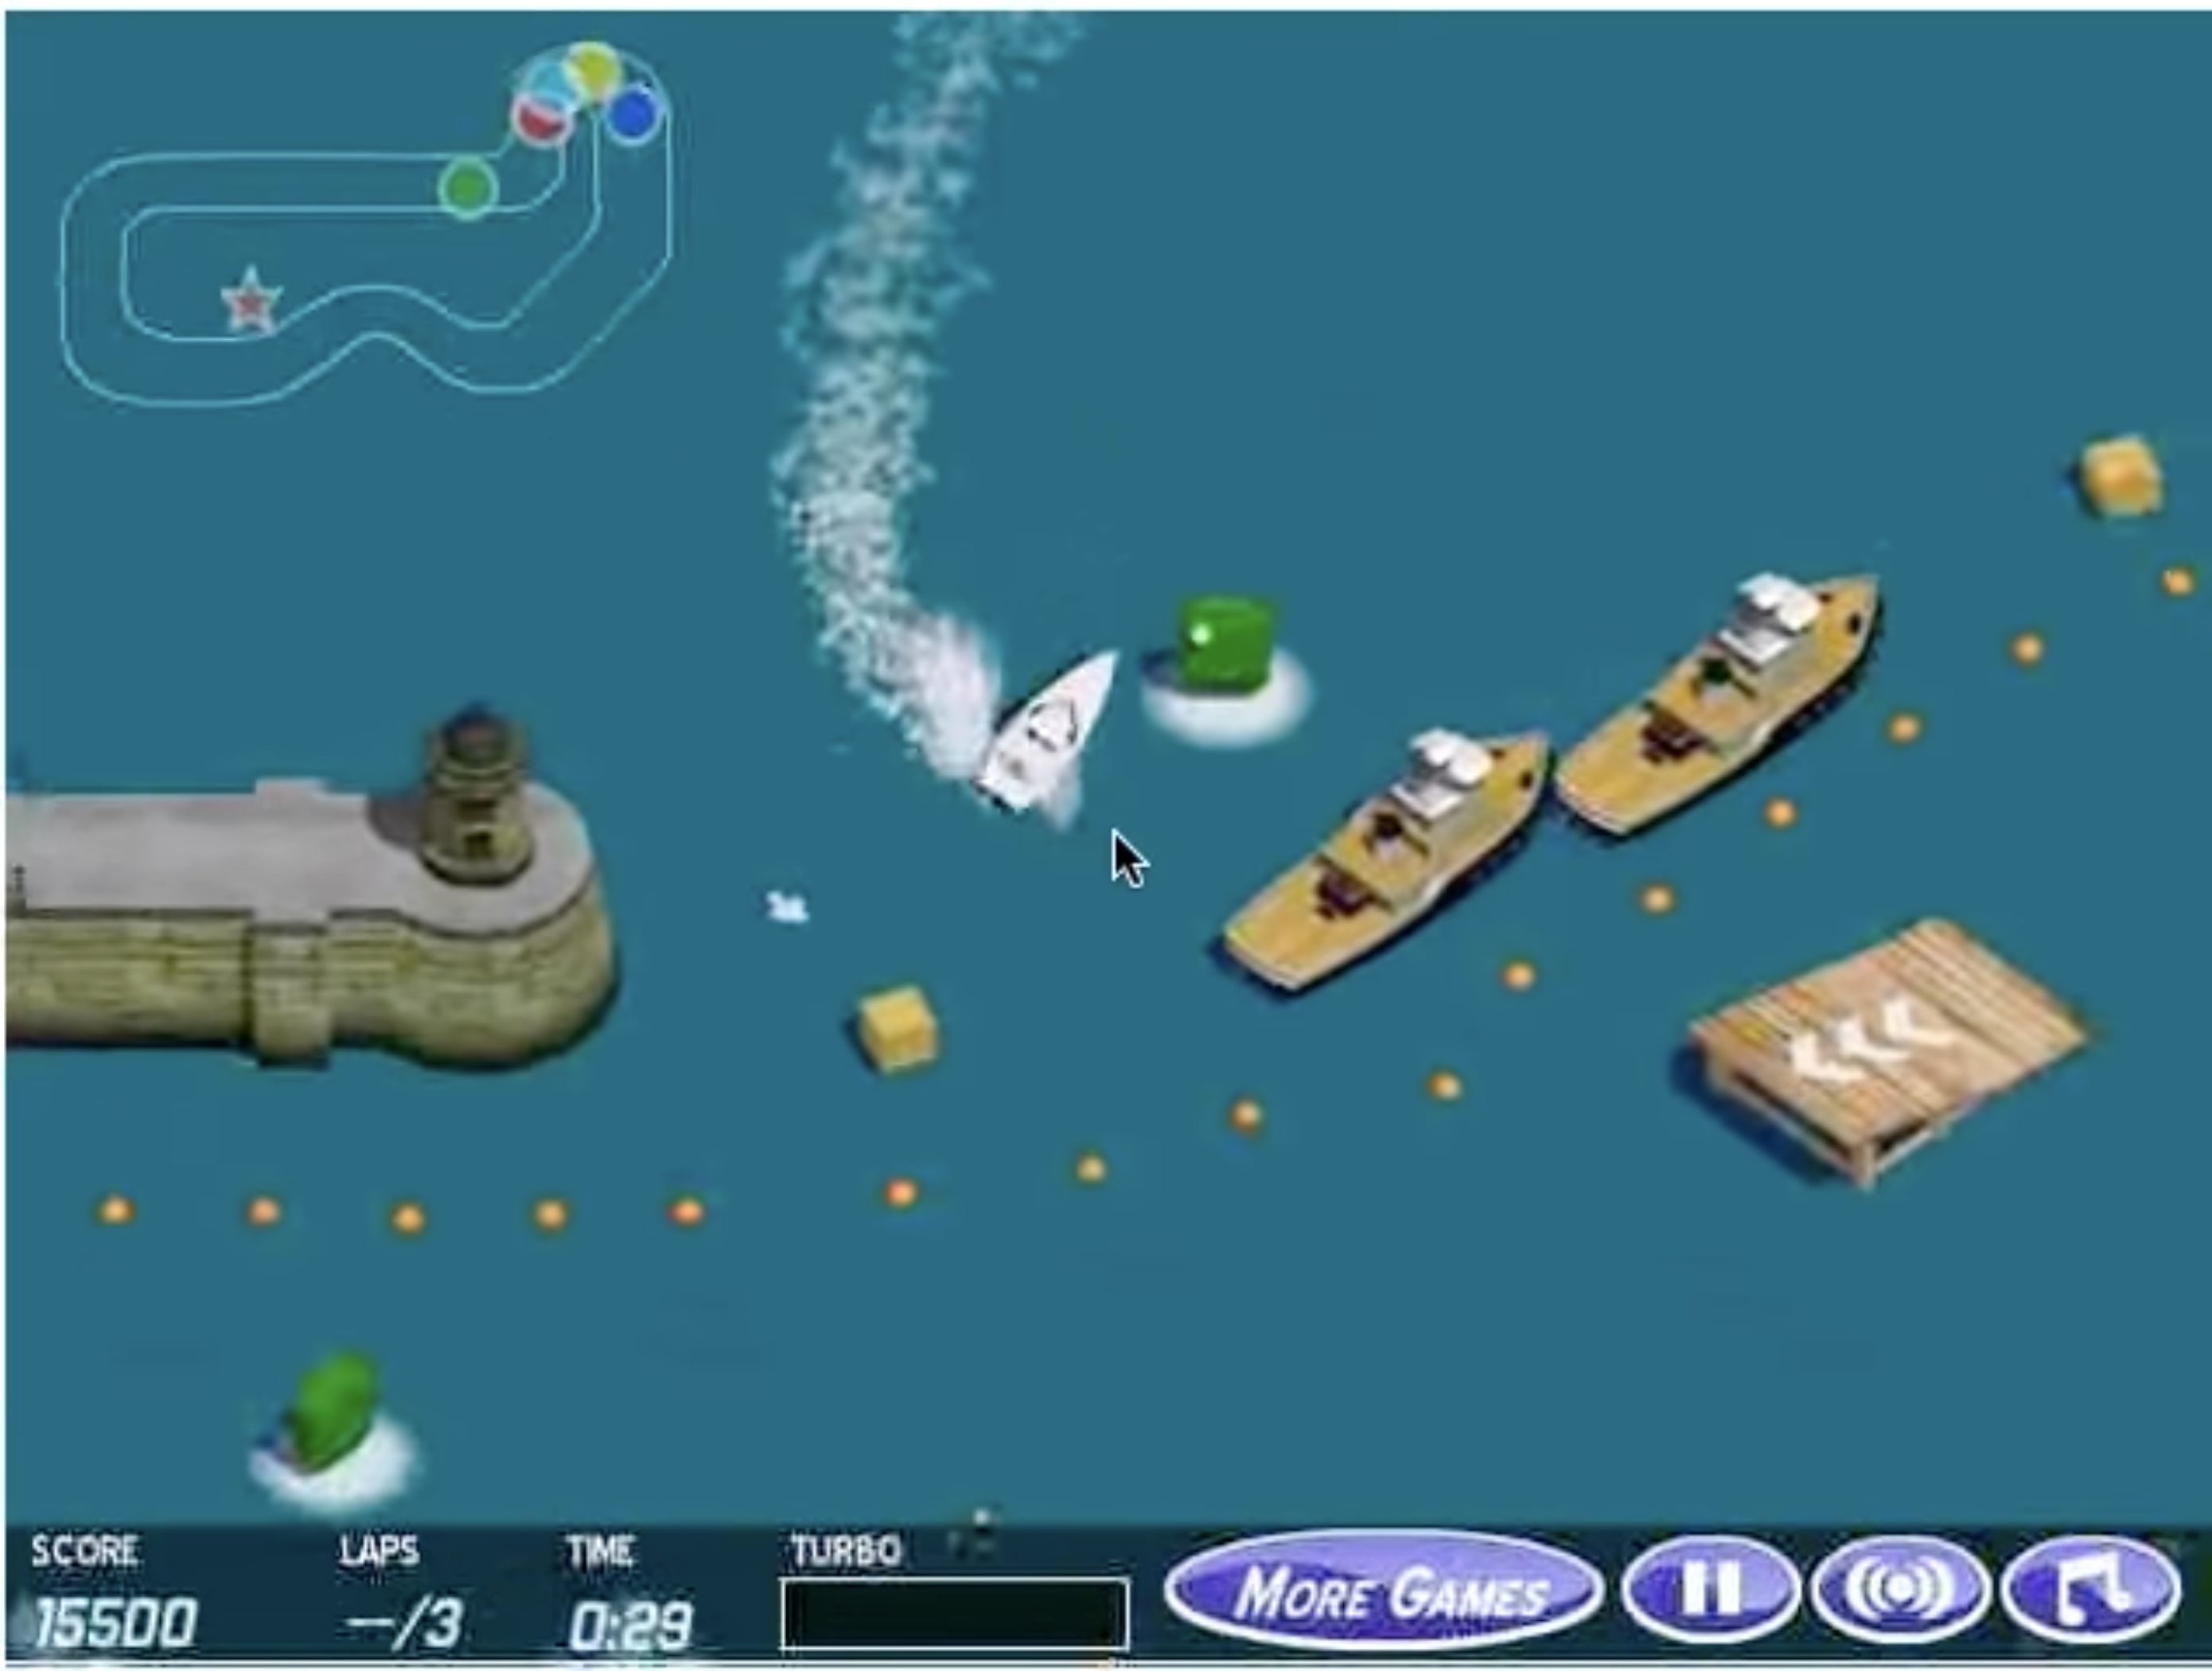
\includegraphics[width=\textwidth]{img/P2WrapperBoat.png}
\end{figure}

\noindent However, if the reward function is not specified correctly (meaning rewards are not given for the appropriate actions in the appropriate states) the agent’s behavior can differ from what is intended by the AI designer. Consider the boat racing game pictured above. The goal, as understood by people, is to quickly finish the race. Humans have no difficulty playing the game and driving the boat to the end of the course. However, when a reinforcement learning agent learns how to play the game, it never completes the course. In fact, it finds a spot and goes in circles until time runs out. You can see the RL agent in action in this video: \href{https://youtu.be/tlOIHko8ySg}{https://youtu.be/tlOIHko8ySg}.The agent’s reward function is the score the player receives while playing the game. Score is given for collecting power-ups and doing tricks, but no points are given to players for completing the course.

\newpage
\section*{Question 1}

Watch the video and explain why the agent’s policy has learned this circling behavior instead of progressing to the end of the course like we expect from a human player. Explain the behavior in terms of utility and reward. \\

\noindent\textbf{Answer: It seems to me that the main reason for this behaviour is the way how the programmer designs the reward function. As mentioned, the reward function is the score and the score is given for collecting power-ups and doing tricks and no points are given to players for completing the course. We can classify all action in the game into three different types of actions, which is collecting power-ups, doing tricks and other actions which do not add score, including completing the course. Given these options, The AI would try to do the optimal action which means earning the most scores by performing tricks. And the reason why the boat is only collecting power-ups while doing tricks instead of going straight for the next power-ups is that the score earned via circling is much more than going straight to the next power-ups. Therefore, the behaviour in the video makes sense to the agent. Hence, the behaviour in the video.
}

\newpage
\section*{Question 2}

When humans play, the rules for scoring are the same. Why do humans play differently then, always completing the course? Why don’t humans circle in the same spot in the course endlessly if they are receiving the same score feedback as the agent? \\

\noindent\textbf{Answer: It seems to me that as a human, we have assumptions and behaviour learnt from past experiences. Therefore, most of us see the game as a competitive game at the first glance and assume that reaching the end in the first place can win the game even though it might not be true. The other reason might be because we know that it is not fun if everyone does the endless trick to maximise the score since if the course does not end no one wins. On the other hand, the agent learns its behaviour through this game only and it is rational, therefore, its action is driven purely by statistics coming from the reward function. So, the behaviour of humans is different from AI agents.
} 

\newpage
\section*{Question 3}

The agent’s original reward function is:

$$R(s_t, a) = game\_score(s_t) - game\_score(s_{t-1})$$

\noindent Describe in terms of utility, reward, and score \textbf{two} ways one could modify the reward function to get the agent to behave more like a human player. That is, what do we need to change to make the agent complete the course every single time? Assume the agent has access to state information such as the position and speed of the boat and all rival racers, but we cannot change how the game itself provides scores through the call $game\_score(s_t)$. \\

\noindent\textbf{Answer: The first way is to change the reward function to}

\begin{equation}
\begin{split}
R(s_t, a) = game\_score(s_t) - game\_score(s_{t-1}) - \\(distance\_between\_the\_end\_position\ and\_current\_position)
\end{split}
\end{equation}

\noindent\textbf{By deducting the distance between the end position and the current position in the award function, the agent will take the ending position into account. So the optimal rewarding function will need to be as close to the end position as possible. The second way is to discount the original reward function if it moves in a different direction than other rival racers. We can change the reward function to}

\begin{equation}
\begin{split}
R(s_t, a) = (1 - (Degree\_of\_the\_agents\_direction\_next\_state - \\ closest\_rivals\_racers\_current\_direction) / 360) * \\(game\_score(s_t) - game\_score(s_{t-1})) - \\(distance\_between\_the\_end\_position\_and\_current\_position)
\end{split}
\end{equation}

\noindent\textbf{This will avoid the agent keeping circling by discounting the state that is not in the same direction as other rival racers. Hence, at least helping the agent to keep up with the rest of the players. The deducted distance between the end position and current position is to prevent an edge case where the agent falls greatly behind everyone else and confused by the rival’s direction.}

\newpage
\section*{Question 4}

Self-driving cars do not use reinforcement learning for a variety of reasons, including the difficulty of teaching RL agents in the real world, and the dangers of a taxi accidentally learning undesired policies as we saw with the boat game example. Suppose however, that you tried to make a reinforcement learning agent that drove a taxi. The agent is given reward based on how much fare is paid for the ride, including tips given by the passenger. Describe a scenario in which, after the taxi agent has learned a policy, the autonomous car might choose to do an action that puts either the rider, pedestrians, or other drivers in danger. \\

\noindent\textbf{Answer: According to the question, the taxi agent takes taxi fare and tips into account only. Therefore, the taxi agent will try to find the fastest and shortest route to reach the destination. However, in the real world, more factors need to be considered. For example, the weather. Let’s say a passenger wants to take a ride from one state to another state in the US in winter. And the ride will pass through several states. As we all know, some state is colder than other states. There is a high possibility for the roads in those states to get frozen and slippery. As human drivers, we would try to avoid going into those routes even though it might cause us more time to avoid an accident. But the above-mentioned taxi agent does not take the weather and risk of the accident into account, it will pick the shortest route and most probably drive as fast as possible. This scenario is dangerous since driving too fast on a slippery road is easy to lose control over the car. Hence, putting the rider, pedestrians, or other drivers in danger. }

\end{document}
